\documentclass[allowframebreaks,aspectratio=169]{beamer}
\usetheme{Execushares}
\mode<presentation>
\colorlet{noir}{black!90!white}
\colorlet{blanc}{white!90!black}
\colorlet{rouge}{red!90!black}
\colorlet{vert}{green!90!black}
\colorlet{bleu}{blue!90!black}
\setbeamercolor{background canvas}{bg=noir}
\setbeamercolor{normal text}{fg=blanc,bg=noir}
\setbeamercolor{structure}{fg=rouge!20!-bleu}
\setbeamercolor{alerted text}{fg=-bleu}
\setbeamercolor{item}{fg=structure.fg}
\setbeamercolor{block title}{fg=blanc,bg=bleu!60!blanc}
\setbeamercolor{block body}{bg=noir!90!blanc}
\setbeamercolor{block title alerted}{bg=rouge!55!noir,fg=blanc}
\setbeamercolor{block body alerted}{bg=noir!90!blanc}
\setbeamercolor{block title example}{bg=-rouge!45!blanc,fg=blanc}
\setbeamercolor{block body example}{bg=noir!90!blanc}
\setbeamercolor{palette primary}{bg=noir,fg=blanc}
\setbeamercolor{palette secondary}{bg=noir,fg=structure.fg}
\setbeamercolor{palette tertiary}{bg=noir,fg=alerted text.fg}
\setbeamercolor{palette quaternary}{bg=noir,fg=bleu!20!blanc}
\setbeamercolor{sidebar}{use=block body, bg=block body.bg}
\setbeamercolor{palette sidebar primary}{use=titlelike, bg=titlelike.bg, fg=titlelike.fg}
\setbeamercolor{section in sidebar}{use=titlelike, fg=titlelike.fg, bg=titlelike.bg}
\setbeamercolor{section in sidebar shaded}{ fg=bleu!20!blanc}
\setbeamercolor{section in head/foot shaded}{fg=bleu!20!blanc}
\setbeamercolor{subsection in sidebar}{use=titlelike, fg=titlelike.fg, bg=titlelike.bg}
\setbeamercolor{subsection in sidebar shaded}{fg=bleu!20!blanc}
\setbeamercolor{subsection in head/foot shaded}{fg=bleu!20!blanc}
\setbeamercolor{logo}{use=block title, bg=block title.bg}
\setbeamercolor{separation line}{fg=blanc,bg=blanc}
\mode<all>

\usepackage{tikz}
\usetikzlibrary{positioning}
\usetikzlibrary{calc}
 \usepackage{emoji}
 
 \usepackage{mdframed}
\usetikzlibrary{arrows}
\usetikzlibrary{decorations, decorations.text,backgrounds}
\definecolor{foreground}{RGB}{255,255,255}
\definecolor{background}{RGB}{24,24,24}
\definecolor{title}{RGB}{107,174,214}
\definecolor{gray}{RGB}{155,155,155}
\definecolor{subtitle}{RGB}{102,255,204}
\definecolor{hilight}{RGB}{102,255,204}
\definecolor{vhilight}{RGB}{255,111,207}
\setbeamercolor{titlelike}{fg=title}
\setbeamercolor{subtitle}{fg=subtitle}
\setbeamercolor{institute}{fg=gray}
\setbeamercolor{normal text}{fg=foreground,bg=background}
\setbeamertemplate{footline}{%
    \raisebox{5pt}{\makebox[\paperwidth]{\hfill\makebox[20pt]{\color{gray}
          \scriptsize\insertframenumber}}}\hspace*{5pt}}
\definecolor{skyblue}{RGB}{215,235,242}
\definecolor{tribor}{RGB}{236,90,50}
\definecolor{vio}{RGB}{164,117,169}
\definecolor{darkpink}{RGB}{245,168,150}
\definecolor{darkvio}{RGB}{125,47,132}
\definecolor{darkblue}{RGB}{3,34,97}
\definecolor{lightblue}{RGB}{94,183,200}
\definecolor{red}{RGB}{255, 0, 0}
\definecolor{blue}{RGB}{0, 118, 186}
\definecolor{green}{RGB}{0,255,0}
\definecolor{gray}{RGB}{146, 146, 146}
\definecolor{colorA}{RGB}{96, 34, 59}
\definecolor{colorB}{RGB}{140, 151, 154}
\definecolor{secinhead}{RGB}{249,196,95}
\definecolor{titlebg}{RGB}{51,51,51}
\definecolor{draculabg}      {RGB} {40,   42,   54}
\definecolor{draculacl}      {RGB} {68,   71,   90}
\definecolor{draculafg}      {RGB} {248,  248,  242}
\definecolor{draculacomment} {RGB} {98,   114,  164}
\definecolor{draculacyan}    {RGB} {139,  233,  253}
\definecolor{draculagreen}   {RGB} {80,   250,  123}
\definecolor{draculaorange}  {RGB} {255,  184,  108}
\definecolor{draculapink}    {RGB} {255,  121,  198}
\definecolor{draculapurple}  {RGB} {189,  147,  249}
\definecolor{draculared}     {RGB} {255,  85,   85}
\definecolor{draculayellow}  {RGB} {241,  250,  140}
\colorlet{draculabrown}{draculared!50!draculared}
\colorlet{red}{draculared}
\colorlet{green}{draculagreen}
\colorlet{blue}{draculacyan}
\colorlet{yellow}{draculayellow}
\colorlet{violet}{draculared}
\colorlet{brown}{draculaorange}
\colorlet{orange}{draculaorange}
\colorlet{cyan}{draculacyan}
\setbeamercolor{titlelike}{fg=rouge!20!-bleu}
\setbeamertemplate{frametitle}{\underline{\textbf{\insertframetitle}}}
% disable navigation
\setbeamertemplate{navigation symbols}{}
%
\AtBeginSection{\frame{\sectionpage}}
\setbeamertemplate{section page}
{
	\begin{tikzpicture}
		% set up the entire slide as the canvas
		\useasboundingbox (0,0) rectangle(\slidewidth,\slideheight);
		%\fill[color=ExecusharesWhite] (0,0) rectangle(\the\paperwidth,\the\paperheight);
		\fill[color=black!90!white] (-1cm, 0cm) rectangle (\slidewidth, \slideheight+0.1cm);
		\node[text width=\the\paperwidth-1cm,align=center] at (0.4\slidewidth, 0.5\slideheight) {\structure{ \Huge\textbf{\insertsection}}};
	\end{tikzpicture}
}


\begin{document}

%\begin{frame}[plain]
	
	
	% Background Image
	\newcommand{\myBackround}
	{
		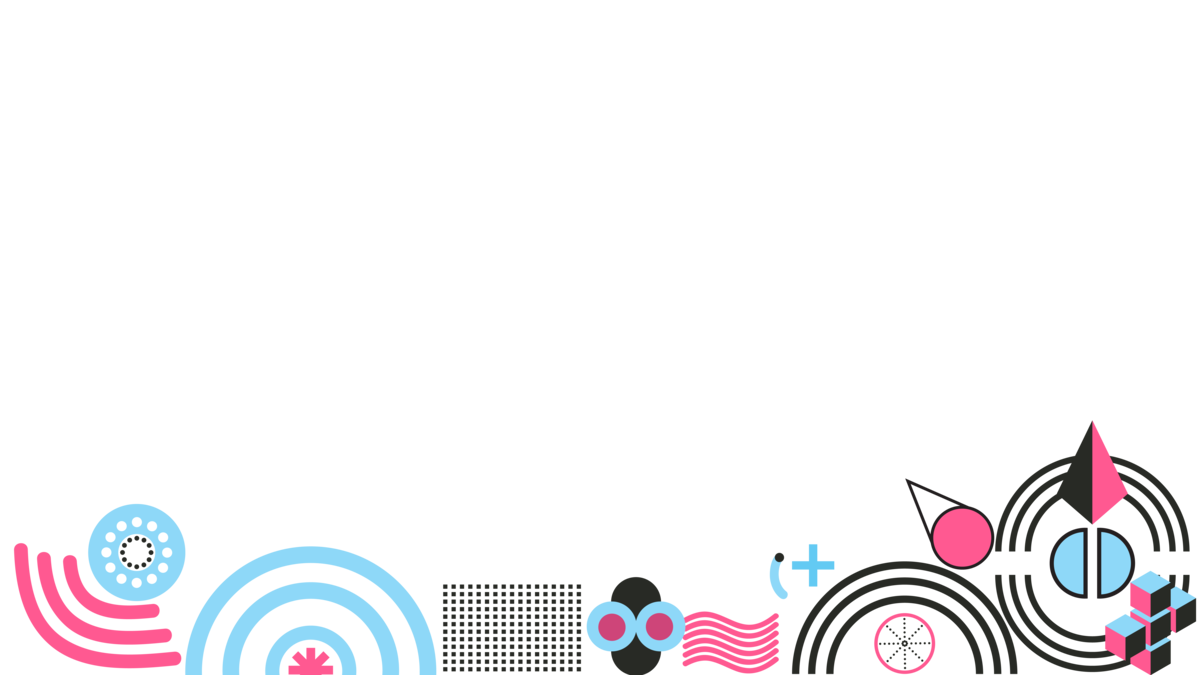
\includegraphics[width=\paperwidth]{Background 5.png}
	}
	
	
	% Title
	\newcommand{\myTitle}
	{
	LES ANNEAUX ,  CORPS ,$\mathbb{Z}$ ,  $\mathbb{Z} / n \mathbb{Z}$
	}
	
	% Subtitle
	\newcommand{\mySubTitle}
	{

	}
	
	% Author
	\newcommand{\myAuthor}   
	{
		Presenté par: \textbf{Groupe 3} \quad\quad\quad Encadré par : \textbf{  Pr. Driss AMRANI}
		
	}
	
	% Affiliation
	\newcommand{\myAffiliate}
	{
		% Affiliation here
	}
	
	% Presentation Date
	\newcommand{\myDate}   
	{
		\today
	}
	
	% Logo
	\newcommand{\myLogo}   
	{
		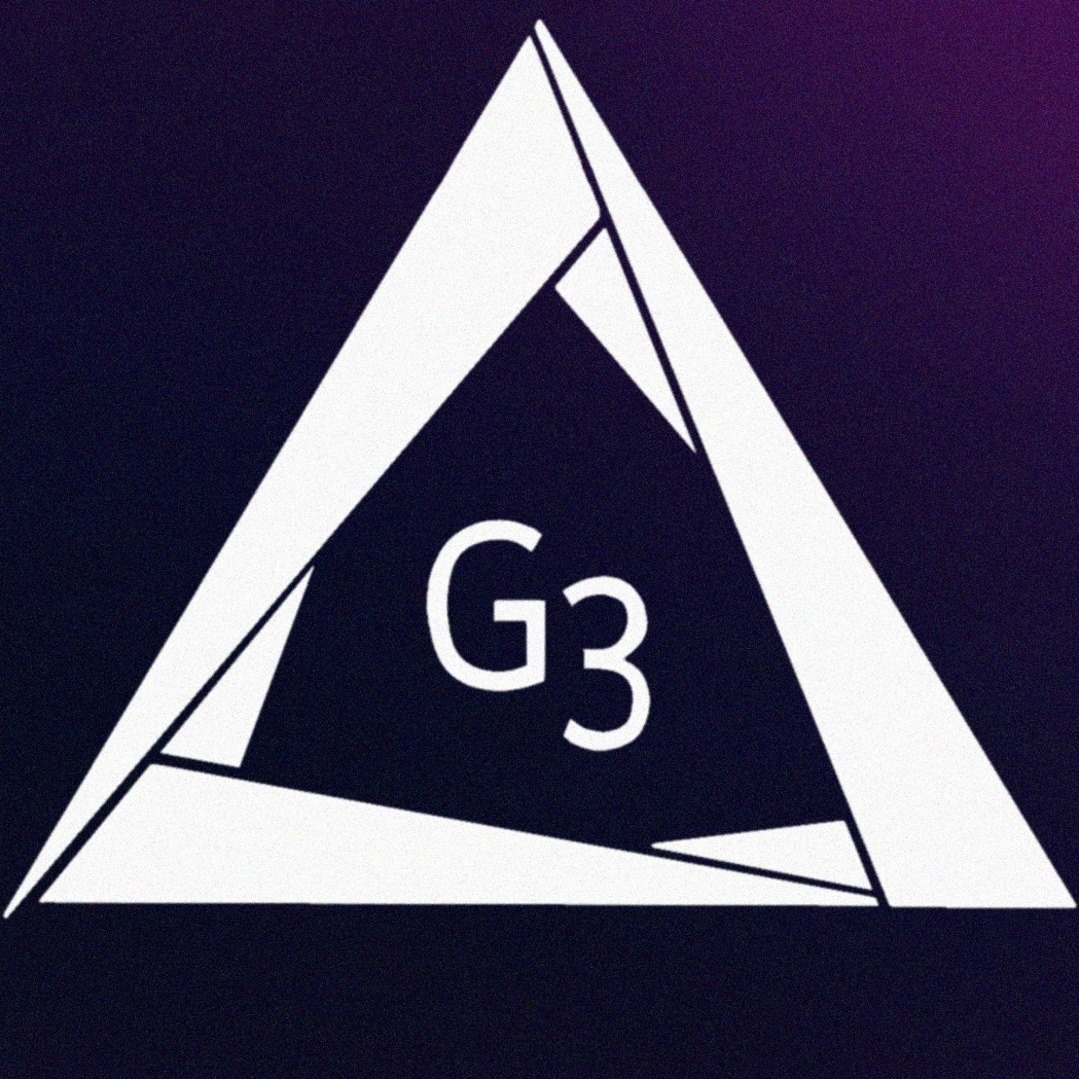
\includegraphics[width=1.5cm]{Beamer-Logo.png}
	}
	%%%%%%%%%%%%%%%%%%%%%%%%%%%%%%%%%%%%
	
	\newcommand{\takwin}   
	{
		
\includegraphics[width=1.7cm]{takwin_logo.jpg}
	}
	
	%%%%%%%%%% Title slide code %%%%%%%%%%%
	\begin{tikzpicture}[remember picture,overlay]
		
		% Background image
		\node[above right,inner sep=0pt] at (current page.south west)
		{
			\myBackround
		};
		
		% Title & Subtitle
		\node
		[
		above=0.5cm,
		align=center,
		fill=bleu!70,
		rounded corners,
		inner xsep=15pt,
		inner ysep=10pt, 
		minimum width=0.7\textwidth,
		text width=0.6\textwidth
		] (title) at (current page.center)
		{
			\LARGE \myTitle 
			\small \mySubTitle
		};
		
		% Author 
		\node[ below=0.3cm] (author) at (title.south){\myAuthor};
		\node[ below left =0.9cm and 0.5cm] (author) at (title.south){Ahmidany fatiha  \quad\quad};
		\node[ below left =1.5cm and 0.2cm ] (author) at (title.south){El Alaoui abdelkarim  \quad\quad};
		\node[ below left =2.1cm and 0.8cm ] (author) at (title.south){Ezzaki ismail  \quad\quad};
		\node[ below left =2.7cm and 0.6cm ] (author) at (title.south){Larbaoui hajar \quad\quad };
		
		
		% Logo
		\node
		[
		below right =0.25cm and 0.5cm
		] at (current page.north west)
		{
			\myLogo
			
			
		};
		
		\node
		[
		below left =0.25cm and 0cm
		] at (current page.north east)
		{
			\takwin
			
			
		};
		
		% Logo
		\node
		[
		below right =2cm and 0.5cm
		] at (current page.north west)
		{
			Groupe 3
			
			
		};
		
	\end{tikzpicture}
	
\end{frame}



\section{Pourquoi apprendre geogebra}
  	\begin{frame}
	\begin{center}
		\structure{
			\Huge{13 reasons why
		}}
	\end{center}
	
	\begin{enumerate}
			\item la géométrie en 2D \pause  et en 3D \pause
		
		\item pas uniquement la géométrie \pause algèbre , probabilités et statistique
				\item pas uniquement les figures \pause exercices / exams / activities
		\pause
				\item économiser du temps + ATP \pause
		\item Geogebra  fonctionnent bien avec le latex
				\pause
				
		\item Math  \emoji{neutral-face}  \quad\quad\quad \pause Math + PC / Phone  \emoji{smiling-face-with-heart-eyes}
		\pause
		
		\item auto-apprentissage 
				\pause
						\item  capacité d'attention
				\pause
		\item un exemple dynamique $= \infty $ exemples
			\pause
		\item moins d'abstraction en mathématiques \pause
		\item La science dit que
\pause
		\item vous n'avez pas besoin de DATASHOW
	\end{enumerate}
\end{frame}
%
%\section{Pourquoi apprendre geogebra}
%\begin{frame}{}
%	\begin{block}{DFINITION}
%		Un anneau est un ensemble muni de deux LCI $(A,+, .)$ tels que :
%		\begin{itemize}
%			\item $(A,+)$ est un groupe commutatif de neutre noté $0_{A}$.
%			\item La loi . est une LCI sur $A$ associative et distibutive à gauche et à droite par rapport à $+$ :  $$ \forall x, y, z \in A, \quad x .(y+z)=x . y+x . z \quad \text { et } \quad(x+y) . z=x . z+y . z $$
%%			\item La loi . admet un neutre différent de $0_{A}$, noté $\mathbf{1}_{A}$.
%		\end{itemize}
%		Si la loi . est commutative, l'anneau est dit commutatif ou abélien.
%	\end{block}
%	\begin{block}{EXERCICE}
%		Si $x \in A$, montrer que $0_{A} \cdot x=0_{A}$ (considérer $0_{A} \cdot x+0_{A} \cdot x$ ).
%	\end{block}
%\end{frame}
%\begin{frame}{}
%	\begin{block}{EXEMPLES}
%		\begin{itemize}
%			\item 		- $(\mathbb{Z},+, .),(\mathbb{Q},+, .),(\mathbb{R},+, .)$ et $(\mathbb{C},+, .)$ sont des anneaux bien connus.
%			\item 		- L'ensemble des suites réelles, muni de l'addition et du produit des suites, est un anneau. Même chose pour l'ensemble des fonctions de $I$ dans $\mathbb{R}$. On déterminera précisément les neutres de ces anneaux.
%		\end{itemize}
%	\end{block}
%\end{frame}
%
%\section{Sous-anneaux}
%\begin{frame}{}
%	\begin{block}{DFINITION}
%		Soit $(A,+, .)$ un anneau. Une partie non vide $A_{1}$ de $A$ est un sous-anneau de $A$ lorsque :
%		\begin{itemize}
%			\item 	- $\mathbf{1}_{A} \in A_{1}$;
%			\item 	- les lois $+$ et . induisent des LCI sur $A_{1}$, et, muni de ces lois, $\left(A_{1},+, .\right)$ est un anneau.
%		\end{itemize}
%	\end{block}
%\end{frame}
%\begin{frame}{}
%	\begin{block}{PROPOSITION}
%		Une partie $A_{1}$ non vide de $A$ est un sous-anneau si et seulement si
%		\begin{itemize}
%			\item 		- $\left(A_{1},+\right)$ est un sous-groupe de $(A,+) ;$
%			\item 		- $\mathbf{1}_{A} \in A_{1}$
%			\item 		- induit une LCI sur $A_{1}$.
%		\end{itemize}
%	\end{block}
%\end{frame}
%\begin{frame}{}
%	\begin{block}{EXEMPLES}
%		\begin{itemize}
%			\item 	- Bien entendu, $\mathbb{Z}$ est un sous-anneau de $\mathbb{Q}$ qui est un sous-anneau de...
%			\item - L'ensemble des fonctions dérivables sur I constitue un sous-anneau des fonctions continues sur $I$, qui constitue lui-même un sous-anneau de l'ensemble des fonctions de I dans $\mathbb{R}$.
%			\item - L'ensemble des suites réelles stationnaires est un sous-anneau de $\left(\mathbb{R}^{\mathbb{N}},+, .\right)$, qui est un sous-anneau de $\left(\mathbb{C}^{\mathbb{N}},+, .\right)$
%		\end{itemize}
%	\end{block}
%\end{frame}
%\section{Morphismes d'anneaux}
%\begin{frame}{}
%	\begin{block}{DFINITION}
%		Soient $(A,+, .)$ et $(B,+, .)$ deux anneaux (on note de la même façon les lois de $A$ et $B \ldots$ ). Un morphisme d'anneaux de $A$ vers $B$ est une application de $A$ vers $B$ telle que :
%		\begin{itemize}
%			\item - $f\left(\mathbf{1}_{A}\right)=\mathbf{1}_{B}$
%			\item - pour tout $x, y \in A, f(x+y)=f(x)+f(y)$ et $f(x . y)=f(x) \cdot f(y)$.
%		\end{itemize}
%	\end{block}
%	\begin{block}{EXEMPLES}
%		\begin{itemize}
%			\item 	- $z \mapsto \bar{z}$ réalise un automorphisme d'anneaux de $\mathbb{C}$.
%			\item 	- $f \mapsto f(\pi)$ réalise un morphisme d'anneaux de $\mathbb{R}^{\mathbb{R}}$ sur $\mathbb{R} \mathbb{R}$.
%		\end{itemize}
%	\end{block}
%\end{frame}
%
%\section{Divisibilité}
%\begin{frame}{}
%	\begin{block}{DFINITION}
%		Soit $(A,+, .)$ un anneau commutatif.
%		\begin{itemize}
%			\item - On dit que $x \in A$ est inversible s'il admet un symétrique pour la loi .
%			\item - On dit que $a \neq 0$ divise $b$ s'il existe $c \in A$ tel que $b=c a$. On note $a \mid b$.
%			\item - On dit que $a \neq 0$ est un diviseur de 0 s'il existe $b \neq 0$ tel que $a b=0$.
%			\item - Un anneau est dit intègre s'il ne contient pas de diviseur de 0 autre que 0 lui-même.
%		\end{itemize}
%	\end{block}
%	\begin{block}{PROPOSITION}
%		Dans un anneau commutatif $(A,+, .)$ :
%		\begin{itemize}
%			\item 	- $0_{A}$ n'est jamais inversible.
%			\item 		- Si $x_{1}, x_{2}, y \in A$ intègre, avec $y \neq 0$ et $x_{1} y=x_{2} y$, alors $x_{1}=x_{2} .$ On dit qu" on peut simplifier" (ce qui ne veut pas dire diviser) par $y \neq 0$.
%		\end{itemize}
%	\end{block}
%\end{frame}
%\begin{frame}
%	\begin{block}{EXEMPLES}
%		-\begin{itemize}
%			\item  $\mathbb{Z}$ est intègre, et ses éléments inversibles sont 1 et $-1 .$
%			\item - Q, $\mathbb{R}$ et C sont des anneaux intègres dont tous les éléments non nuls sont inversibles.
%			\item - L'ensemble des fonctions de $\mathbb{R}$ dans $\mathbb{R}$ n'est pas intègre : toute application $f$ qui s'annulle est diviseur de 0 (le montrer). Les éléments inversibles sont les fonctions qui ne s'annullent pas.
%		\end{itemize}
%	\end{block}
%	\begin{block}{EXERCICE}
%		Montrer que $\mathbb{Z}[i]=\{a+b i \mid a, b \in \mathbb{Z}\}$ est un sous-anneau intègre de $\mathbb{C}$, dont les inversibles sont $1, i,-1$ et $-i$.
%	\end{block}
%\end{frame}
%\section{Idéaux}
%\begin{frame}
%	\begin{block}{Définition}
%		on appelle idéal à gauche de l'anneau $A$, un sous-groupe de $(A,+)$ tel que: $$ \forall a\in A  \forall x \in I ax\in I$$
%		on appelle idéal à droite de A un sous groupe de $(A,+)$ tel que:
%		$$\forall a \in A \forall x \in I xa \in I $$
%		On appelle idéal bilatére de $A$ un sous- groupe de $(A,+)$ qui vérifie les deux conditions précédentes.
%	\end{block}
%\end{frame}
%\begin{frame}
%	Évidemment, si l'anneau $A$ est commutatif, les trois notions sont identiques. On dit alors tout simplement, "un idéal" de $A$.
%	Dans un anneau $A$, il existe au moins deux idéaux bilatères, à savoir $\{0\}$ et $A$.\\
%	Supposons $A$ unifere. Pour que $I \neq \varnothing$ soit un idéal à gauche, il suffit que
%	$$\forall x \in I \quad \forall y \in I \quad x+y \in I \quad \text{et} \quad \forall a \in A \quad \forall x \in I \quad a x \in I .$$
%	car alors $0=0 x \in I$ et $-x=(-1) x \in I$ pour tout $x \in I$. Ainsi $I$ est un sous-groupe de $(A,+)$.\\
%	Supposons $A$ unitaire. Si un idéal à gauche (resp. à droite) I de $A$ contient l'unité 1 de $A$, alors $I=A$ car alors $a=a 1 \in I$ pour tout $a \in A$. Plus généralement, si $I$ contient un élément inversible $u$ de $A$, alors $1=u^{-1} u \in I$ et donc $I=A$.\\
%	Un idéal de $A$ est un sous-anneau de $A$ car $(1)$ ou $(2)$, montre que $x y \in I$ pour tout $x \in I$ et tout $y \in I .$ La réciproque est fausse : par exemple $Z$ est un sous-anneau de $\mathbb{R}$ mais n'est pas un idéal de $\mathbb{R}$.\\
%\end{frame}
%\begin{frame}
%	\begin{block}{Prposition}
%		Soit $f: A \longrightarrow B$ un morphisme d'anneaux.\\
%		(i) Soit Jun idéal à gauche (resp. à droite, bilatère) de B. Alors $f^{-1} 1(J)$ est un idéal à gauche (resp. à droite, bilatère) de $A .$
%		En particulier, le noyau $\operatorname{Ker}(f)=f^{-1}(\{0\})$ de $f$ est un idéal bilatère de $A$.\\
%		(ii) Supposons $f$ surjectif. L'image $f(I)$ de tout idéal à gauche (resp. à droite, bilatère) I de $A$, est un idéal à gauche (resp. à droite, bilatère) de $B$.\\
%		(iii) Supposons $f$ surjectif. L'application $\alpha: J \mapsto f^{-1}(J)$ est une bijection, de 1 'ensemble $\mathcal{J}$ des idéaux bilatères de $B$ sur l'ensemble $\mathcal{F}$ des idéaux bilatères de A contenant Ker $(f)$ et $\alpha$ respecte l'inclusion.
%	\end{block}
%\end{frame}
%\begin{frame}
%	\begin{proof}
%		(i) $f^{-1}(J)$ est un sous-groupe additif de $A$. Pour $x \in f^{-1}(J)$ et $a \in A$ on a $f(x) \in J$, d'où $f(a x)=f(a) f(x) \in J$ et donc $a x \in f^{-1}(J)$.\\
%		(ii) Nous laissons la vérification au lecteur.\\
%		(iii) D'après (i), si $J$ est un idéal bilatère de $B$, alors $f^{-1}(J)$ est un idéal bilatère de $A .$ Il contient Ker $(f)=f^{-1}(\{0\}) .$ Ainsi $\alpha$ est une application de $\mathcal{J}$ dans $\mathcal{F} .$ Si $J, J^{\prime} \in \mathcal{J}$ sont tels que $J \subset J^{\prime}$ on a $f^{-1}(J) \subset f^{-1}\left(J^{\prime}\right)$ donc $\alpha$ respecte l'ordre. Pour tout $J \in \mathcal{J}$ on a $f\left[f^{-1}(J)\right]=J$ car $f$ est surjective donc $\alpha$ est injective. Elle est surjective car pour tout $I \in \mathcal{F}$, on a Ker $(f) \subset I$ et donc $f^{-1}(f(I))=I+\operatorname{Ker}(f)=I .$
%	\end{proof}
%\end{frame}
%\section{Intersection et somme d'idéaux}
%\begin{frame}
%	\begin{block}{Proposition}
%		$\|$ Soit $\left(I_{k}\right)_{k \in K}$ une famille d'idéaux à gauche de l'anneau $A$.
%		(i) $\bigcap_{k \in K} I_{k}$ est un idéal à gauche de $A$.
%		(ii) L'ensemble $\sum_{k \in K} I_{k}$ des éléments $x \in A$ qui sont somme finie $x_{i_{1}}+\cdots+x_{i_{k}}$ d'éléments de $\bigcup_{K \in K} I_{k}$, est un idéal à gauche de A. C'est le plus petit idéal à gauche de A contenant $I_{k}$ pour tout $k \in K$.
%		En particulier, la somme $I+J=\{x+y ; x \in I, y \in J\}$ de deux idéaux à gauche $I$ et Jde $A$, est un idéal à gauche de $A .$
%	\end{block}
%\end{frame}
%\section{Quotient d'un anneau par un idéal bilatère}
%\begin{frame}
%	\begin{block}{Lemme}
%		Soient $A$ un anneau, I un sous-groupe du groupe additif $(A,+)$. La relation d'équivalence de congruence modulo le sous-groupe I,
%		$$
%			x \equiv y \Leftrightarrow y-x \in I,
%		$$
%		est compatible avec le produit de $A$, si et seulement si I est un idéal bilatère de $A$.
%	\end{block}
%\end{frame}
%\begin{frame}
%	\begin{proof}
%		L'équivalence est compatible avec les multiplications à gauche, si pour $x, y \in A$, la condition $x \equiv y$ implique que $a x \equiv$ ay pour tout $a \in A$, soit si pour tout $z \in I$ et tout $a \in A$, on a $a z \in I$, c'est-à-dire si $I$ est idéal à gauche.
%		De même, l'équivalence est compatible avec le produit du côté droit si et seulement si $I$ est un idéal à droite de $A$, d'où le lemme.
%	\end{proof}
%\end{frame}
%\begin{frame}
%	\begin{block}{Proposition}
%		Soient $A$ un anneau et $I$ un idéal bilatère de $A$. Le quotient $A / I$, muni des opérations
%		$$
%			\bar{x}+\bar{y}=\overline{x+y} \quad, \quad \bar{x} \bar{y}=\overline{x y}
%		$$
%		est un anneau. Si $A$ a une unité, alors $\overline{1}$ est une unité pour $A / I$.
%		L'application canonique $\varphi: x \mapsto \bar{x}$ est un homomorphisme d'anneaux surjectif de $A$ sur $A / I$, de noyau $I$ et le couple $(A / I, \varphi)$ a la propriété universelle suivante (factorisation des homomorphismes):
%		(P) Si un homomorphisme fde A dans un anneau B est nul sur I, alors il existe un homomorphisme unique $\bar{f}: A / I \rightarrow B$ tel que $\bar{f} \circ \varphi=f$.
%		De plus, on a $\operatorname{Im}(\bar{f})=\operatorname{Im}(f)$ et $\operatorname{Ker}(\bar{f})=\operatorname{Ker}(f) / I$.
%	\end{block}
%\end{frame}
%\begin{frame}
%	\begin{proof}
%		$A / I$ est un groupe additif. D'après le lemme, le produit est bien défini sur $A / I$ et les axiomes des anneaux sont vérifiés (voir 1-2).
%		Soit $f \in \operatorname{Hom}(A, B)$ nul sur $I$.
%		on définit un homomorphisme de groupes additifs en posant $\bar{f}(\bar{x})=\overline{f(x)}$ pour tout $\bar{x} \in A / I$. On a
%		$$
%			\bar{f}(\overline{x y})=\bar{f}(\overline{x y})=f(x y)=f(x) f(y)=\bar{f}(\bar{x}) \bar{f}(\bar{y}),
%		$$
%		donc $\bar{f}$ est un homomorphisme d'anneaux, d'où la propriété universelle $(\mathrm{P})$.
%	\end{proof}
%\end{frame}
%\section{ Idéaux maximaux}
%\begin{frame}
%	\begin{block}{Définition}
%		On appelle idéal a gauche maximal de 1 ' anneau $A$, un idéal a gauche I de $A$, distinct de $A$, tel que les seuls idéaux à gauche de $A$ contenant I soient I et A. On définit de même les notions d 'idéal à droite maximal et d 'idéal bilatère maximal.
%	\end{block}
%\end{frame}
%\begin{frame}
%	\begin{block}{Proposition}
%		Soit $A$ un anneau avec unité.
%		Tout idéal à gauche de $A$, distinct de $A$, est inclus dans un idéal à gauche maximal. Tout idéal à droite de $A$, distinct de $A$, est inclus dans un idéal à droite maximal. Tout idéal bilatère de $A$, distinct de $A$, est inclus dans un idéal bilatère maximal.
%	\end{block}
%\end{frame}
%\section{ Corps}
%\begin{frame}
%	\begin{block}{Définition}
%		Un corps est un anneau $K$, possédant une unité 1 (distincte du zéro) tel que tout élément non nul $x$ possède un inverse $x^{-1}$.
%		Si le produit est commutatif, on dit que $K$ est un corps commutatif.
%		On appelle sous-corps de $K$ un sous-anneau $K_{0}$ de $K$ contenant $l^{\prime}$ unité de $K$ et tel que pour tout $x \in K_{0}$ non nul on ait $x^{-1} \in K_{0}$.
%	\end{block}
%	Un corps $K$ est donc un anneau unitaire dont le groupe des unités est $K_{*}=\mathrm{K} \backslash\{0\}$.
%	Un corps est intègre : si $x y=0$ et si $x \neq 0$ alors $x$ est inversible et $y=x^{-1}(x y)=0$.
%	L'intersection d'une famille $\left(K_{i}\right)_{i \in I}$ de sous-corps d'un corps $K$ est non seulement un sous-anneau de $K$ contenant l'unité mais c'est un sous-corps de $K$. En effet, pour tout $x \in \bigcap_{i \in I} K_{i}$, avec $x \neq 0$, on a $x^{-1} \in K_{i}$ pour tout $i \in I$ et donc $x^{-1} \in \bigcap_{i \in I} K_{i}$.
%	Soit $X$ une partie non vide de $K$. L'intersection des sous-corps de $K$ contenant $X$, est le plus petit sous-corps de $K$ contenant $X$, appelé le sous-corps engendré par $X$.
%	Les corps $Q, R, C$ jouent un rôle essentiel en mathématique.
%\end{frame}
%\begin{frame}
%	\begin{block}{Proposition}
%		Soit $K$ un anneau avec unité. Pour que $K$ soit un corps, il faut et il suffit que $\{0\}$ et $K$ soient les seuls idéaux à gauche de $K$. Il en est de même pour les idéaux à droite.
%	\end{block}
%\end{frame}
%\begin{frame}
%	\begin{proof}
%		Soit $I$ un idéal à gauche du corps $K .$ Si $I \neq\{0\}$, il existe $x \in I$ non nul. On a $1=x^{-1} x \in I$ et donc $I=K$.
%		Réciproquement, soit $K$ un anneau unitaire ayant pour seuls idéaux à gauche $\{0\}$ et $K$. Pour tout $x \neq 0$ l'idéal à gauche $K x$ de $K$ contient $x$. Il est donc égal à $K$. En particulier, il existe $y \in K$ tel que $y x=1$. Comme $y \neq 0$, il existe de même $z \in K$ tel que $z y=1$. Alors $y$ qui a un inverse à droite $x$ et un inverse à gauche $z$, est inversible d'inverse $y^{-1}=x$. Tout élément non nul $x$ de $K$ est donc inversible et $K$ est un corps.
%		On montre de même l'assertion concernant les idéaux à droite.
%	\end{proof}
%\end{frame}
%\section{Quotient par un idéal maximal}
%\begin{frame}
%	\begin{block}{Proposition}
%		Soit A un anneau commutatif unitaire. Pour qu'un idéal I de A soit maximal, i1 faut et il sufiit que A/I soit un corps.
%	\end{block}
%\end{frame}
%\begin{frame}
%	\begin{proof}
%		l'anneau commutatif unitaire $A / I$ est un corps si et seulement si $\{0\}$ et $A / I$ sont ses seuls idéaux. D'après , prop. (iii), cela signifie que $I$ et $A$ sont les seuls idéaux de $A$ contenant 1, c'est-à-dire que $I$ est maximal.
%	\end{proof}
%\end{frame}
%\begin{frame}
%	\begin{block}{Corollaire}
%		$\|$ L'anneau $\mathbb{Z} / p \mathbb{Z}$ est un corps si et seulement si $p \in N$ est premier.
%	\end{block}
%\end{frame}
%\section{Construction de l'ensemble $\mathbb{Z}$ des entiers relatifs}
%\begin{frame}{}
%	\begin{center}
%		\textbf{Pourquoi on applle les entiers relatifs $\mathbb{Z}$}
%		\begin{itemize}
%			\item $ \mathbb{N}  \Rightarrow $ Nombre
%			\item $ \mathbb{R}  \Rightarrow $ Reel
%			\item $ \mathbb{C}  \Rightarrow $ Complexe
%			\item $ \mathbb{Z}  \Rightarrow $ \pause Nombre en allemand \textbf{{\color{red} Zahlen}}
%		\end{itemize}
%	\end{center}
%\end{frame}
%\begin{frame}{}
%	Normalement, en utilisant les nombres naturels, on peut facilement définir les entiers relatifs comme suit :
%	Les \textbf{ entiers relatifs}, notés $\mathbb{Z}$, sont tous les nombres entiers positifs et négatifs : soit
%	\begin{align*}
%		\mathbb{Z} = \{ \ldots -2, -1, 0, 1, 2, 3, \ldots\}.
%	\end{align*}
%	Cependant, on peut facilement voir que la définition ci-dessus est suspecte,
%	\begin{itemize}
%		\item Que signifie $-3$ ?
%		\item Comment $-3$ interagit-il avec l'addition et la multiplication ?
%		\item nous n'avons pas de règles qui équivalent à "vous pouvez faire une deuxième copie de votre premier ensemble mais avec des symboles spéciaux devant tous ces éléments"
%	\end{itemize}
%\end{frame}
%\begin{frame}[allowframebreaks]{classes d'équivalence}
%	Prenons un ensemble quelconque $S$ avec une relation d'équivalence $R$.  Pour tout élément $x \in S$, nous pouvons définir la \textbf{classe d'équivalence} correspondant à $x$ comme l'ensemble
%	\begin{align*}
%		\{y \in S ~|~ y R x\}
%	\end{align*}
%	Par exemple, dans l'arithmétique pour modulo 3 il existe trois classes d'équivalence possibles :
%	\begin{align*}
%		\{ \ldots -6, -3, 0, 3, 6 \ldots\} \\
%		\{ \ldots -5, -2, 1, 4, 7 \ldots\} \\
%		\{ \ldots -4, -1, 2, 5, 8 \ldots\} \\
%	\end{align*}
%	Chaque élément correspond à l'une de ces trois classes.
%\end{frame}
%\begin{frame}{Définir $\mathbb{Z}$}
%	En utilisant ce concept, nous définissons les entiers relatifs comme suit :
%	\pause
%	\begin{block}{définition}
%		Construire $\mathbb{N} \times \mathbb{N} = \mathbb{N}^2$, le produit cartésien des nombres naturels par eux-mêmes.  Créer une relation d'équivalence $\sim$ sur $\mathbb{N} \mathbb{N}$ de la manière suivante :
%		\begin{itemize}
%			\item 		écrivez $(a,b) \sim (c,d)$ si et seulement si $a-b = c-d$. ( $(a,b) \sim (c,d)$ si et seulement si $a+d = b+c$ ; ceci est équivalent).
%			\item 		Prenez la collection de toutes les classes d'équivalence de $\mathbb{N}^2$ sous cette relation.  Nous appelons cet ensemble le \textbf{entiers relatifs}, et l'écrivons $\mathbb{Z}$.
%		\end{itemize}
%	\end{block}
%\end{frame}
%\begin{frame}{Définir $\mathbb{Z}$}
%	\begin{columns}
%		\begin{column}{0.3\linewidth}
%			\pause[1]
%			$\bullet~$	{\color{blue} $(a,b)$ correspond à l'entier $a-b$, où notre relation d'équivalence est une façon de dire que $(a,b)$ et $(a+k, b+k)$ représentent tous deux le même "entier relatif"}.\vspace{1em}
%			\pause[3]{
%				$\bullet~${\color{red} 	Cela peut sembler bizarre, mais cela a l'avantage d'être un ensemble que nous pouvons etudier (c'est une collection de sous-ensembles de $\mathbb{N}^2$).  }
%			}
%		\end{column}
%		\begin{column}{0.6\linewidth}
%			\pause[2]
%			\begin{center}
%				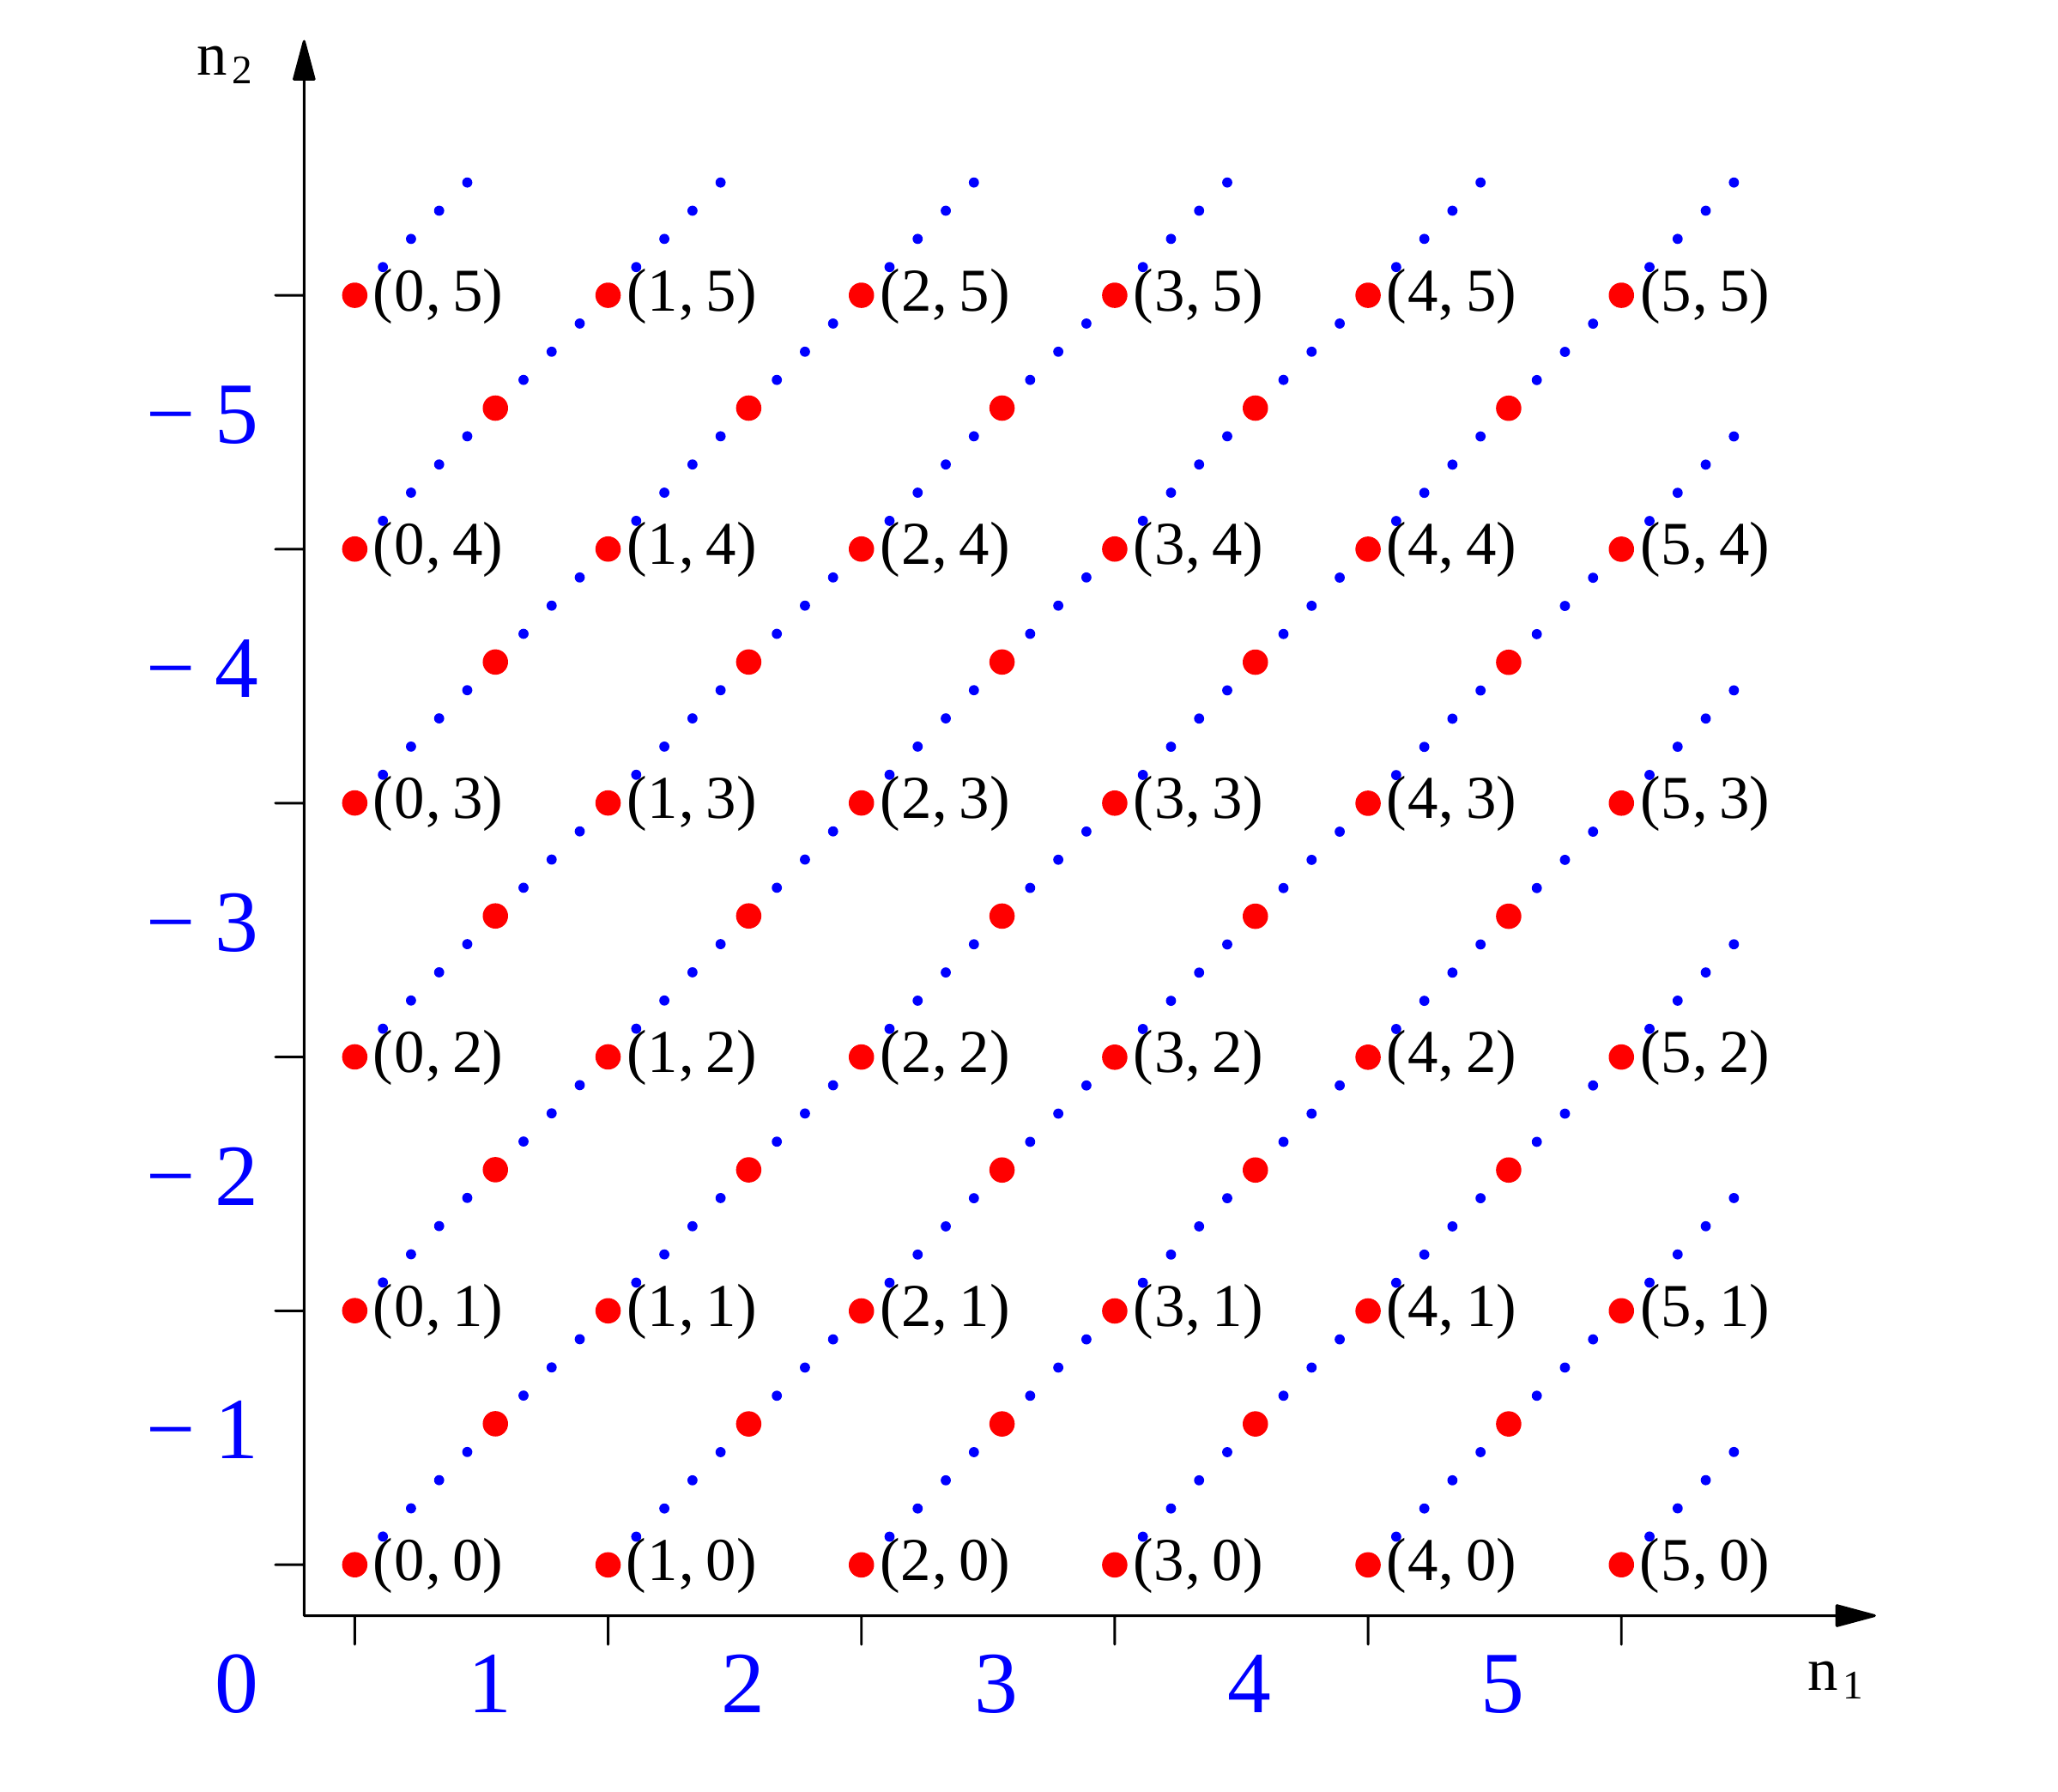
\includegraphics[width=\linewidth]{geo/image1}
%			\end{center}
%		\end{column}
%	\end{columns}
%\end{frame}
%\begin{frame}{Définition de la structure de groupe}
%	\begin{center}
%		\textbf{L'addition}
%	\end{center}
%	\begin{itemize}
%		\item On définit la somme de deux couples d'entiers ainsi : $ (n_{1},n_{2})+(n_{1}',n_{2}')=(n_{1}+n_{1}',n_{2}+n_{2}') $; cette opération est commutative, associative et d'élément neutre $(0,0)$ sur les couples d'entiers , dont le neutre est la classe de $(0,0)$, constituée des couples $(n,n)$.
%		\item si $(n_{1},n_{2}) $ représente un entier relatif dans les couples d'entiers, ${\displaystyle (n_{1},n_{2})+(n_{2},n_{1})} = (n_{1}+n_{2},n_{1}+n_{2})$ donc équivalent à $(0,0)$. $\Rightarrow$ La classe d'équivalence de $(n_{2},n_{1})$ est donc opposée à la classe d'équivalence de $(n_{1},n_{2})$.
%		\item   Il existe une classe d'équivalence $Z$ contenant cette paire, car les classes d'équivalence partitionnent $\mathbb{N}^2$ !
%		\item    Remarquez que le représentant choisi n'a pas d'importance, car choisir n'importe quel autre représentant $(n_1 + c, n_2 + c), (n_{1}'+d, n_{2}' + d)$ donnerait $(n_{1} + n_{2}+c+d, n_{1}'+n_{2}'+c+d),$ ce qui est équivalent à $(n_1+n_{1}', n_2+n_{2}')$, il s'agit d'une opération bien définie !
%	\end{itemize}
%\end{frame}
%\begin{frame}{Définition de la structure de groupe}
%	\begin{center}
%		\textbf{L'addition}
%	\end{center}
%	\begin{center}
%		\begin{columns}
%			\begin{column}{0.5\linewidth}
%				\begin{center}
%					\begin{mdframed}[backgroundcolor=blue!50,linecolor=blue!50]
%						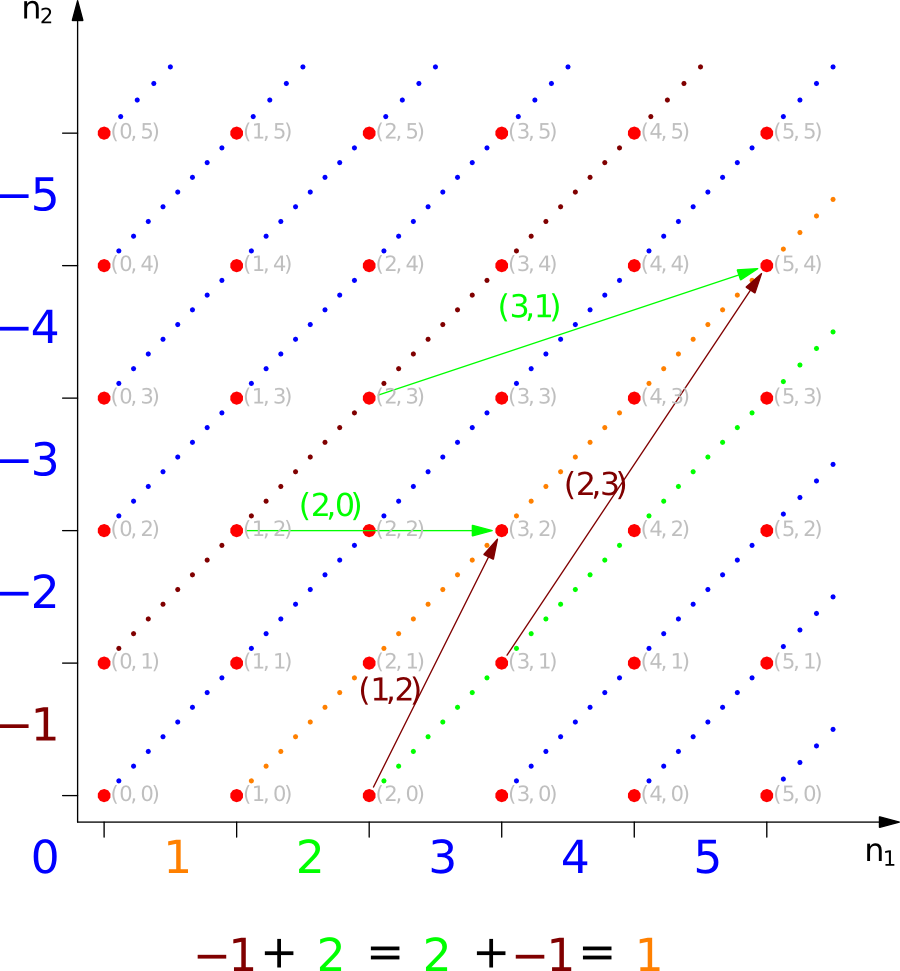
\includegraphics[width=\linewidth]{geo/IntegerAddition}
%					\end{mdframed}
%				\end{center}
%			\end{column}
%		\end{columns}
%	\end{center}
%\end{frame}
%\begin{frame}{Définition de la structure de groupe}
%	\begin{center}
%		\textbf{ la multiplication}
%	\end{center}
%	On peut alors définir la multiplication comme suit : ${\displaystyle (n_{1},n_{2})\times (m_{1},m_{2})=(n_{1}m_{1}+n_{2}m_{2},n_{1}m_{2}+m_{1}n_{2})}$
%	Cette opération définie sur ${\displaystyle \mathbb {N} \times \mathbb {N} }$ est associative, commutative, possède un élément neutre (1, 0) et est distributive pour l'addition précédemment définie. De plus, elle donne à ${\displaystyle \mathbb {Z} }$ une structure d'anneau unitaire.
%	Les égalités
%	\begin{itemize}
%		\item ${\displaystyle (d,0)\times (d',0)=(dd',0)}$
%		\item ${\displaystyle (d,0)\times (0,d')=(0,dd')}$
%		\item ${\displaystyle (0,d)\times (0,d')=(dd',0)}$
%	\end{itemize}
%	permettent les écritures
%	\begin{itemize}
%		\item ${\displaystyle d\times d'=dd'}$
%		\item ${\displaystyle d\times (-d')=(-dd')}$
%		\item ${\displaystyle (-d)\times (-d')=dd'}$
%	\end{itemize}
%	qui permettent de démontrer que l'anneau est aussi intègre.
%\end{frame}
%\begin{frame}{Définition de la structure de groupe}
%	\begin{center}
%		\textbf{ la relation d'ordre}
%	\end{center}
%	Pour comparer deux classes d'équivalence quelconques $X,Y$:
%	\begin{itemize}
%		\item choisissez un représentant $(x_1,x_2) \in X, (y_1,y_2) \in Y$.
%		\item 	On dit que $X < Y$ si et seulement si $x_1 - x_2 < y_1 -y_2$, ou de manière équivalente $x_1 + y_2 < y_1 + x_2$.
%		\item 	Là encore, on peut vérifier que cette propriété ne dépend pas des représentants choisis dans les classes d'équivalence de $X,Y$, donc elle aussi est bien définie.
%	\end{itemize}
%\end{frame}
%\begin{frame}{Écriture simplifiée des éléments de Z}
%	Notons (n ; m) la classe d'un couple d'entiers naturels (n, m). Elle est de l'un des trois types suivants :
%	\begin{itemize}
%		\item $(d ; 0)$ si $n > m$ avec $n = m + d$ et $d$ non nul
%		\item $(0 ; d)$ si $n < m$ avec $n + d = m$ et $d$ non nul
%		\item $(0 ; 0)$ si $n = m$
%	\end{itemize}
%	Or l'ensemble des classes (d ; 0) est isomorphe à ${\displaystyle \mathbb {N} }$  ; on note donc ces classes sous la forme simplifiée d.
%	D'autre part, pour d non nul, les classes (d ; 0) et (0 ; d) sont opposées. En effet, (d ; 0) + (0 ; d) = (d ; d) = (0 ; 0). On note donc les classes (0 ; d) sous la forme simplifiée (–d).
%	L'ensemble ${\displaystyle \mathbb {Z} }$ retrouve alors sa forme plus classique de ${\displaystyle \mathbb {N} \cup \{(-d)\mid d\in \mathbb {N} ^{*}\}}$.
%\end{frame}
%\begin{frame}{Propriétés de $\mathbb{Z}$}
%	Les entiers satisfont toutes les propriétés énumérées précédemment pour $\mathbb{N}$, à l'exception du bon ordre :
%	\begin{itemize}
%		\item \textbf{stabilité($+$)}: $\forall a, b \in \mathbb{Z},$ on a $a+b \in \mathbb{Z}$.
%		\item \textbf{Identité($+$)}: $\exists 0 \in \mathbb{Z}$ tel que $\forall a \in \mathbb{Z}$, $0+a = a$.
%		\item \textbf{Commutativité($+$)}: $\forall a, b \in \mathbb{Z}, a+b = b+a$.
%		\item \textbf{Associativité($+$)}: $\forall a, b, c \in \mathbb{Z}, (a+b)+c = a+(b+c)$.
%		\item  \textbf{stabilité($\cdot$)}: $\forall a, b \in \mathbb{Z},$ on a $a\cdot b \in \mathbb{Z}$.
%		\item \textbf{Identité($\cdot$)}: $\exists 1 \in \mathbb{Z}$ tel que $\forall a \in \mathbb{Z}$, $\cdot a = a$.
%		\item \textbf{Commutativité($\cdot$)}: $\forall a, b \in \mathbb{Z}, a\cdot b = b \cdot a$.
%		\item \textbf{Associativité($\cdot$)}: $\forall a, b,c \in \mathbb{Z}, (a\cdot b)\cdot c =a \cdot(b \cdot c)$.
%		\item \textbf{Distributivité}: $\textbf{(}+,\cdot\textbf{)}: \forall a, b,c \in \mathbb{Z}, (a+ b)\cdot c =(a \cdot c)+ (b\cdot c)$
%	\end{itemize}
%	En outre, il satisfait aux deux propriétés supplémentaires suivantes :
%	\begin{align*}
%		 & \bullet~ \text{Inverses}\textbf{(}+\textbf{)}: \forall a \in \mathbb{Z}, \exists \textrm{ a unique } (-a) \in \mathbb{Z} \textrm{ tel aue }a + (-a) = 0. \\
%		 & \bullet~ \text{Ordre  de  multiplication(}<,\cdot\textbf{)}: \forall a,b,c \in \mathbb{Z},\textrm{ si }a < b, 0 < c\textrm{ alors }ac < bc.
%	\end{align*}
%\end{frame}
%\begin{frame}{	Proposition : L'anneau $(\mathbb{Z},+, *)$ }
%	Le triplet $(\mathbb{Z},+, *)$ est un anneau commutatif , intègre et unitaire
%\end{frame}
%\begin{frame}{$\mathbb{N} , \mathbb{R}, \mathbb{C}$}
%	\begin{center}
%		pour approfondir : la construction de $\mathbb{N} , \mathbb{R}, \mathbb{C}$
%	\end{center}
%	$
%		https://web.math.ucsb.edu/~padraic/ucsb\_2014\_15/ccs\_proofs\_f2014/ccs\_proofs\_f2014.html
%	$
%\end{frame}
%\section{L'anneau $\mathbb{Z} / n \mathbb{Z}$}
%\begin{frame}
%	\textbf{	Congruences dans $\mathbb{Z}$}\\
%	Soit $n$ un entier naturel.\\
%	\textbf{	Rappels} Nous avons vu en première année la relation de congruence modulo $n$ définie par :
%	$$
%		x \equiv y \quad[n] \Longleftrightarrow y-x \in n \mathbb{Z} .
%	$$
%\end{frame}
%\begin{frame}
%	Il s'agit d'une relation d'équivalence sur $\mathbb{Z}$ qui est compatible arec les opérations de $\mathbb{Z}$, c'est-à-dire qui vérifie :
%	$$
%		\forall\left(x, y, x^{\prime}, y^{\prime}\right) \in \mathbb{Z}^{4}\left\{\begin{array} { l l }
%			{ x \equiv x ^ { \prime } } & { [ n ] } \\
%			{ y \equiv y ^ { \prime } } & { [ n ] }
%		\end{array} \Longrightarrow \left\{\begin{array}{ll}
%			x+y \equiv x+y^{\prime}                        & {[n]}   \\
%			x \times y \equiv z^{\prime} \times y^{\prime} & {[n] .}
%		\end{array}\right.\right.
%	$$
%	\textbf{	Notation}
%	On note $\mathbb{Z} / n \mathbb{Z}$ l'ensemble des classes d'équivalence pour cette relation.
%	La classe d'un élément $k$ de $\mathbb{Z}$ est notée $\bar{k}$.\\
%\end{frame}
%\begin{frame}
%	\begin{block}{Proposition}
%		Pour $n \in \mathbb{N}^{*}$, l'ensemble $\mathbb{Z} / n \mathbb{Z}$ a $n$ éléments, et l'on a :
%		$$
%			\mathbb{Z} / n \mathbb{Z}=\{\overline{0}, \overline{1}, \ldots, \overline{n-1}\}
%		$$
%	\end{block}
%	\textbf{Remarque} $\mathbb{Z} / n \mathbb{Z}$ est appelé ensemble quotient de $\mathbb{Z}$ par $n \mathbb{Z}$, ce qui explique sa notation.
%\end{frame}
%\begin{frame}
%	\begin{block}{Proposition}
%		1. Il existe sur $\mathbb{Z} / n \mathbb{Z}$ des lois, notées $+$ et $\times$ (ou implicitement pour le produit) et appelées lois quotient, telles que :
%		$\forall(x, y) \in(\mathbb{ Z} / n \mathbb{Z})^{2} \quad \bar{x}+\bar{y}=\overline{x+y}$ et $\bar{x} \times \bar{y}=\overline{x y} .$
%		2. $(\mathbb{Z} / n \mathbb{Z},+, x)$ est un anneau commutatif d'éléments neutres $\overline{0}$ et $\overline{1}$.\\
%		3. La projection canonique $\mathbb{Z} \rightarrow \mathbb{Z} / n \mathbb{Z}$ est un morphisme d'anneaux surjectif de noyau $n \mathbb{Z}$.
%	\end{block}
%\end{frame}
%\begin{frame}
%	\begin{block}{Remarque}
%		- On peut aussi prendre pour représentants des classes modulo $n \neq 0$, n'importe quel $n$-uplet d'entiers consécutifs.\\
%		Par exemple, pour étudier la multiplication sur $\mathbb{Z} / 5 \mathbb{Z}$, il pourra être intéressant d'écrire $\mathbb{Z} / 5 \mathbb{Z}=\{\overline{0}, \pm \overline{1}, \pm \overline{2}\} .$\\
%		- Les éléments $0,1, \ldots, n-1$ sont privilégiés dans leurs classes respectives. Il arrivera donc que l'on note $p$ à la place de $\bar{p}$ lorsque $0 \leqslant p<n, s^{\prime}$ il n'y a pas de confusion possible.
%	\end{block}
%\end{frame}
%\begin{frame}
%	\begin{block}{Proposition}{(Éléments inversibles de $\mathbb{Z} / n \mathbb{Z}$ )}
%		1. La classe de $k \in \mathbb{Z}$ est inversible dans $\mathbb{Z} / n \mathbb{Z}$ si, et seulement $s i, k$ est premier avec $n$.\\
%		2. Pour $n \in \mathbb{N}^{*}$, les assertions suivantes sont équivalentes :
%		(i) $\mathbb{Z} / n \mathbb{Z}$ est un corps;\\
%		(ii) $\mathbb{Z} / n \mathbb{Z}$ est intègre;\\
%		(iii) $n$ est premier.
%	\end{block}
%\end{frame}
%\section{Théoréme chinois}
%\begin{frame}
%	On note ici $[k]_{n}$ la classe de l'entier $k$ modulo un entier naturel non nul $n .$
%	\begin{block}{Proposition}
%		Soit $n$ et $m$ des entiers premiers entre eux. Les anneaux $\mathbb{Z} /(n m) \mathbb{Z}$ et $(\mathbb{Z} / n \mathbb{Z}) \times(\mathbb{Z} / m \mathbb{Z})$ sont isomorphes par le morphisme d'anneaux $\varphi:$
%		$$
%			\begin{aligned}
%				\mathbb{Z} /(n m) \mathbb{Z} & \longrightarrow(\mathbb{Z} / n \mathbb{Z}) \times(\mathbb{Z} / m \mathbb{Z}) \\
%				{[k]_{n m} }                 & \longrightarrow\left([k]_{n},[k]_{m}\right)
%			\end{aligned}
%		$$
%	\end{block}
%\end{frame}
%\begin{frame}
%	\begin{block}{Corollaire}  {(Théorème chinois)}
%		Si $n$ et $m$ sont des entiers premiers entre eux, pour tout $(a, b) \in \mathbb{Z}^{2}$, il existe un entier $k$ vérifiant le système:
%		$$
%			\begin{cases}k \equiv a & {[n]} \\ k \equiv b & {[m]}\end{cases}
%		$$
%		et les solutions de ce système sont exactement les entiers congrus à $k$ modulo $n m$.
%	\end{block}
%\end{frame}
%\begin{frame}
%	Le théorème chinois permet de ramener l'étude d'une équation sur $\mathbb{Z} / n \mathbb{Z}$ lorsque $n$ n'est pas premier, à celle d'équations sur des anneaux plus simples.\\
%	\textbf{Point méthode (pour obtenir une solution de $(S)$ )}
%	A partir d'une relation de Bézout $n u+n v=1$, on trouve deux entiers $k_{1}=m u$ et $k_{2}=n v$ vérifiant respectivenent les systemes de congruences:
%	$$
%		\begin{cases}k_{1} \equiv 1 & {[n]} \\ k_{1} \equiv 0 & {[m]}\end{cases}
%	$$
%	et
%	$$
%		\begin{cases}k_{2} \equiv 1 & {[n]} \\ k_{2} \equiv 0 & {[m]}\end{cases}
%	$$
%	et une solution du systèe $(S)$ est alors $k=k_{1} a+k_{2} b$ (vérification imme diate en prenant les congruences nodulo $n$ et $m)$
%	\textbf{	Remarque }L'obtention d'une telle solution est non triviale, mais sa vérification est immédiate. Il ne faut donc pas oublier de la faire pour repérer une erreur de calcul éventuelle.
%\end{frame}
%
%
%{
%	\setbeamertemplate{background} 
%	{
%		
\includegraphics[width=\paperwidth,height=\paperheight]{06-six-more-orange-circles}
%	}
%	\begin{frame}[c]
%		
%		
%		\centering
%		\Huge{ Merci pour votre Attention ?}
%		
%		
%		
%		
%	\end{frame}
%}

\end{document}
